\documentclass[12pt,a4paper]{article}

\usepackage[utf8x]{inputenc}
\usepackage[english]{babel}
\usepackage{xcolor}
\usepackage{hyperref}
\usepackage{parskip}
\usepackage{graphicx}
\usepackage{listings} % For code snippets
\usepackage{xcolor}
\usepackage[left=2cm, top=3cm, text={17cm, 24cm}]{geometry} 

\definecolor{codegreen}{rgb}{0,0.6,0}
\definecolor{codegray}{rgb}{0.5,0.5,0.5}
\definecolor{codepurple}{rgb}{0.58,0,0.82}
\definecolor{backcolour}{rgb}{0.95,0.95,0.92}

% Setup for code snippets
\lstdefinestyle{mystyle}{
    backgroundcolor=\color{backcolour},   
    commentstyle=\color{codegreen},
    keywordstyle=\color{magenta},
    numberstyle=\tiny\color{codegray},
    stringstyle=\color{codepurple},
    basicstyle=\ttfamily\footnotesize,
    breakatwhitespace=false,         
    breaklines=true,                 
    captionpos=b,                    
    keepspaces=true,                 
    numbers=left,                    
    numbersep=5pt,                  
    showspaces=false,                
    showstringspaces=false,
    showtabs=false,                  
    tabsize=4
}

% Path to images
\graphicspath{ {./images/} } 

% Setup for hyperrefs
\hypersetup{
    colorlinks=true,
    linkcolor=blue,
    filecolor=magenta,      
    urlcolor=blue,
}

% TODO command
\newcommand{\todo}[1]{\textcolor{red}{\textbf{[[TODO]]}} $\Rightarrow$ \textbf{#1}}
% Globally disable indentation -> package parskip
\setlength{\parindent}{0pt}

\begin{document}
    \begin{titlepage}
        \begin{center}
            \vspace*{1cm}
    
            \Large{\textbf{Project ISA}}
    
            \vspace{0.5cm}
            Monitoring of SSL connection
                
            \vspace{1.5cm}
            
            \textbf{Pavel Yadlouski (xyadlo00)}
    
            \vfill
                
            \vspace{0.8cm}
        
            Brno University of Technologies\\
            September, 2020
                
        \end{center}
    \end{titlepage}
    
    \tableofcontents
    \newpage

    \section{Introduction}
    This project aims to create simple CLI application, that can monitor SSL communication.
    Here monitoring means to aggregate input file \textbf{and/or} given network interface.  
        

    \section{Architecture}
    \begin{center}
        \begin{figure}[h!]
            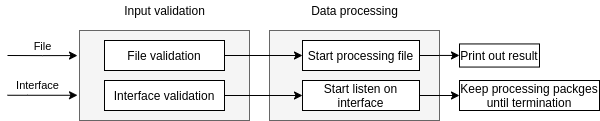
\includegraphics[scale=0.7]{sslsniff.png}
        \end{figure}
    \end{center}
    The whole program contains two main parts:
    \begin{enumerate}
        \item input validation
        \begin{enumerate}
            \item check if file exists and with supported extension
            \item check if given interface exists and can be opened for listening
        \end{enumerate}
        \item data processing
        \begin{enumerate}
            \item aggregate given file
            \item start live aggregation of incoming traffic on given interface
        \end{enumerate}
    \end{enumerate}
    The result of file aggregation is written to the standard output as soon as
    aggregation is completed. If the interface is set, then the program starts 
    listening on the given interface and aggregate incoming packets. When the 
    last packet of any connection is aggregated, then the result of the 
    aggregation for this particular connection would be written to the standard 
    output. In both cases connection is marked as closed and written to standard
    output if a structure of the connection contains valid SNI attribute and 
    two FIN (from the client and from the server)  

    \subsection{Storing connections}
    As data structure for storing connections information doubly linked list is used.
    This data structure was chosen for its simplicity in implementation and use. 
    Also, despite the hash table, the doubly linked list very flexible from the 
    memory usage point of view: the doubly linked list doesn't have a fixed size, 
    so can grow as much as it would be necessary. The case of resizing the hash 
    table requires recalculating hashes for every item, but the doubly linked list 
    doesn't have this problem. There just insert to any side of the list. Also as 
    each element of the list has a pointer to previous and next elements, then 
    deleting of an element is quite trivial: reset pointers between siblings of 
    given connection and delete the required one.

    The biggest disadvantage of a doubly linked list is high (\textit{O(n)}) 
    searching complexity.For every package whole list can be looked through. 
    But in this application it is not significant, because is very simple. 

    \subsection{Packet processing}

    When the program is started and the first packet comes, then it would be set 
    as the first element in the list. After that for every packet would be found 
    a corresponding entry in the list (based on comparing source and destination 
    IP addresses and ports). If the entry doesn't exist, then this packet would 
    be inserted at the beginning of the list with corresponding linking with next
    element of the list.
    
    Entry for connection is deleted from the list as soon as connection is closed
    (has valid SNI and two FIN flags). With file aggregation, after process of
    aggregation is ended, then list is freed. 


    \subsection{Multithreading}
    Program use separated threads for processing file and interface simultaneously. 
    The main thread would wait first on the file processing thread and then on 
    the interface thread.

    
    \section{Implementation}
    The program contains two parts: checking of input parameters and package 
    aggregation by itself. The first part presents in \textit{sslsniff.c}. Also 
    setup functions for aggregation are called there. The second part is represented 
    in the file \textit{functions.c} with header \textit{functions.h}. 

    There are several auxiliary data structures for packet aggregation. 

    \subsection{TLS extensions}
    For processing SSL/TLS extensions there is following structure
    \lstset{style=mystyle}
    \begin{lstlisting}[language=C]
typedef struct {
    u_int16_t ext_type;
    u_int16_t ext_len;
    char *data;
} extention;
\end{lstlisting}
     
    This structure helps to go through extensions in SSL/TLS headers and find an 
    extension with SNI. 
    To check the type of an extension there is an element \textit{ext\_type}. 
    This value is extracted from the byte stream from corresponding position. 
    Type of extension contains 16 bits, so there is need to convert two following 
    bits, taking into account system byte order. For this purposes (creating 
    unsigned int of 16 bits) there is a function \textit{get\_uint\_16}
    \begin{lstlisting}[language=C]
u_int16_t get_uint_16(u_int8_t *x){
#if __BYTE_ORDER == __LITTLE_ENDIAN
    u_int8_t tmp[2] = {*(x + 1), *x};
#elif __BYTE_ORDER == __BIG_ENDIAN
    u_int8_t tmp[2] = {*x, *(x + 1)};
#endif
    return *(u_int16_t *)tmp;
}
\end{lstlisting}

    This functions is used whenever we need to convert two following bytes to 
    one value with the right byte order.
    Attribute \textit{ext\_len} is used in \textit{for} loop as dynamic step. \
    It is also created with function \textit{get\_uint\_16}. Data of extension
    are stored in \textit{data} attribute.

    So, for extracting the SNI name there is a \textit{for} loop with step 
    \textit{ext\_len} through all extensions. In this
    loop, there is \textit{if} statement which checks the type of extension, and if it
    is equal to 0, then this extension would contain SNI name in its data. In the
    end, if this type of extension presents, SNI is extracted and stored to the
    corresponding element in TLS connection structure.
    
    \subsection{TLS connection}
    Each SSL/TLS connection is represented by the following structure
    \begin{lstlisting}[language=C]
 typedef struct tls_conn{
     u_int src_ip, dst_ip;
     struct in6_addr ip6_src, ip6_dst;
     u_int16_t src_port, dst_port;
     struct timeval timestamp;
     double duration;
     char *sni;
     u_int packet_count;
     u_int bytes;
     u_int addr_size;
     bool server_fin, client_fin, last_ack;
     struct tls_conn *prev, *next;
 } tls_connection;
\end{lstlisting}

    There are the source and destination IP addresses in integer format (for IPv4) 
    and in \textit{ip6\_addr} structure (for IPv6). 
    The reason for storing addresses in an integer format is that comparing integers
    is faster than comparing strings. For comparing IPv6 addresses there is a loop 
    through each byte of address Conversion to human ridable format is 
    made only when the result of aggregation should be written to standard output. 
    Also, for detecting that packet is corresponds to a given connection there 
    are source and destination ports. 

    For aggregation purposes, there are elements for storing the number of packets
    in given connection, duration, and bytes. Durations of connections is founded 
    as a result of subtraction \textit{timestamp} (represents timestamp of the first 
    packet aggregated in given connection) and timestamp of a new packet for 
    corresponding connection. For subsection of timestamps, there is function 
    \textit{time\_diff} 

    For interface aggregation end of the communication is detected based on flags 
    \textit{server\_fin, client\_fin}, and \textit{last\_ack}. These flags correspond 
    to TCP flags of a given connection. The connection is considered closed when 
    flag \textit{last\_ack} is set to \textit{True}. This happens when all of 
    flags \textit{server\_fin} and \textit{client\_fin} also have value \textit{True}. 

    As a doubly linked list is used, then there are also pointers to the next 
    element (connection) and previous. 

    On the step of input validation, the \textit{cleanup} function is set to be 
    triggered on signal \textit{SIGINT}. This step is necessary for interface 
    aggregation. Processing of live connection is not limited, so this setup 
    insure that data will be freed of interruption.

    \section{Problems and limitations}
    \subsection{TCP reassembling}
    Reassembling of TCP packets is not implemented.
    
    \subsection{CPU usage}
    There is a problem that in 1 from cca 10 runs of interface aggregation after a 
    random amount of packets program would load one core up to 100\% and stop 
    writing logs to standard output. The reason for this might be some infinite 
    loop in code, but this problem isn't solved.  

    \subsection{Performance}
    As for storing data during aggregation doubly linked list is used, with a 
    big amount of live connection or on long runs performance of an application 
    is going down due to searching time in the data structure.


    \newpage
    \nocite{*}
    \bibliographystyle{style}
    \bibliography{sample}


\end{document}